\documentclass[12pt,a4paper]{article}
\usepackage{hyperref}

\title{Title} 
\author{Alsayed M., Balducci S., Berselli G., Gargiulo F., Rondini T.}
\date{10/01/2023}

\usepackage{amsmath}
\usepackage{amsfonts}
\usepackage{amssymb}
\usepackage{amsthm}
\usepackage{braket}
\usepackage[margin=3cm]{geometry}
\usepackage{pgfplots}
\pgfplotsset{compat=1.18}
\usepackage{fancyhdr}
\usepackage{physics}
\usepackage{systeme,mathtools}
\usepackage{graphicx}
\usepackage{float}
\usepackage{relsize}
\usepackage{calligra}
\usepackage{siunitx}
\usepackage[miktex]{gnuplottex}
\usepackage{epstopdf}
\usepackage[english]{babel}
\usepackage{csquotes}
\usepackage{float}
\floatplacement{figure}{H}
\usepackage{tikz}
\usetikzlibrary{shapes.misc}
\usepackage[style=ieee]{biblatex}
\addbibresource{biblio.bib}
\usepackage{pgf}
\usepackage{caption}
\usepackage{subcaption}

\newcommand{\R}{\Re}
\newcommand{\la}{\lambda}
\newcommand{\al}{\alpha}
\newcommand{\bd}{\textbf}
\newcommand{\rita}{\longrightarrow}
\newcommand{\lang}{\left\langle}
\newcommand{\rang}{\right\rangle}
\newcommand{\lbra}{\left\lbrace}
\newcommand{\rbra}{\right\rbrace}

\begin{document}

\maketitle
\begin{center}
	\url{https://github.com/Grufoony/Aral_Sea_shrinking}
\end{center}

\begin{abstract}
    Abstract
\end{abstract}
\thispagestyle{empty}

\newpage
\thispagestyle{empty}
\addtocounter{page}{-2}
\mbox{}

\tableofcontents
\pagebreak

\section*{Introduction}
Satellite images are an excellent tool to study landscape’s time evolution both in the long and in the short term and they are freely available in the public domain. 
These are helpful for a wide range of analysis related to human or natural impact on the landscape evolution through time such as urban growth, deforestation, flooding, ice melting, lake shrinking and more. 

In this work we applied image processing’s techniques to multi-temporal satellite images to study the multiannual change of the surface extension of Aral Sea, that was a lake lying between Kazakhstan and the north of Uzbekistan. 
We took the cue from the paper of Vanjare et al. \cite{satelliteImg} in which urban growth of Bangalore region has been studied and discussed by using multi-temporal and multi-spectral Landsat satellite images. 
The aim of this work is to quantify the superficial extension of Aral Sea and its reduction through time due to human activities. We used data from a public archive of the USGS. 
The images are cloudless and of the same resolution, already geo-localized with well-defined coordinates. 
Our analysis is based on simple image processing’s techniques, i.e. image segmentation with a k-mean clustering, thresholding and edge detection.   

The Aral Sea was an endorheic lake lying between Kazakhstan in the north and Uzbekistan in the south which began shrinking in the 1960s and had largely dried up by the 2010s. 
It was formerly the fourth largest lake in the world with a surface area of $68000\,km^2$.  
However, an attempt to grow cottons, melons, rice and cereals in the desert, the so-called Soviet irrigation project, foresaw the deviation of its fed rivers by 1960s. 
From then surface evaporation and lack of rain made the shrinking process rapid. Several attempts were made through time in order to restore the original sea. For example, in $2005$ was completed the building of a dike to prevent the surface extension and the volume of the water in the north basin of the lake, the one lying in Kazakhstan. 
In fact, this side of the lake has nowadays almost the same surface extension than before. 
Unfortunately, the attempts made were not enough: satellite images acquired by NASA in August $2014$ revealed that for the first time in modern history the eastern basin of the Aral Sea had completely dried up. 

\pagebreak

\section{Discussion}
Image processing has revealed as an excellent instrument applied to satellite images. 
In particular, we were able to quantify the shrinking ratio of the Aral Sea during a 44-years timespan by using a combination of techniques, among which k-mean clustering and threshold. 
The result is an almost linear decay, explainable qualitatively by a combination of precipitation/evaporation phenomena.

Furthermore, we were also able to improve a time-evolution visualization by using an edge detection technique and creating an animated GIF.

Observations gathered by multiple earth observation satellites, such as Landsat, combined with the processing techniques serves as a common, reliable record for environmental change around the world. 
Indeed, in the last half century, the record of Earth observation from space has become the indispensable foundation of almost all deliberations about the state of the planet only to study our case, but also to keep track on all kinds of environmental changes which can put us a step ahead of any environmental catastrophe. 


\newpage
\thispagestyle{empty}
\mbox{}

\appendix

\section{Appendix}
\begin{figure}
     \centering
     \begin{subfigure}[b]{0.19\textwidth}
         \centering
         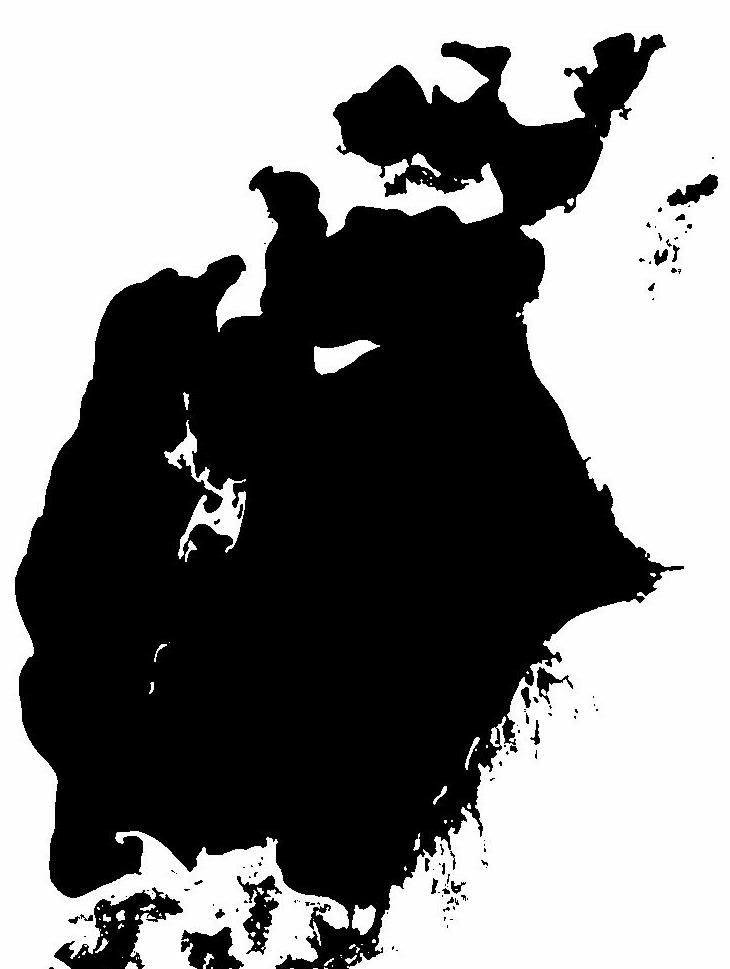
\includegraphics[width=\textwidth]{../img/1977w.jpg}
         \caption{}
         \label{fig:}
     \end{subfigure}
     \begin{subfigure}[b]{0.19\textwidth}
         \centering
         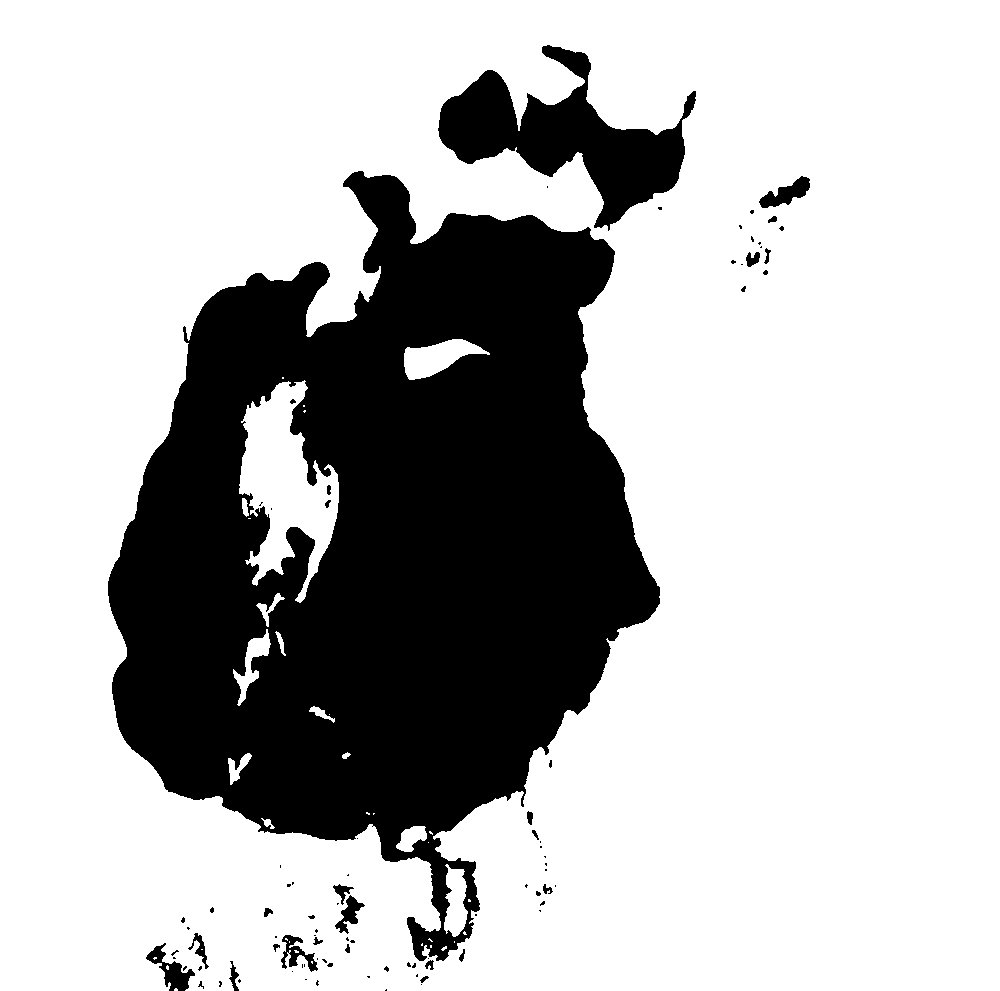
\includegraphics[width=\textwidth]{../img/1987w.jpg}
         \caption{}
         \label{fig:three sin x}
     \end{subfigure}
     \begin{subfigure}[b]{0.19\textwidth}
         \centering
         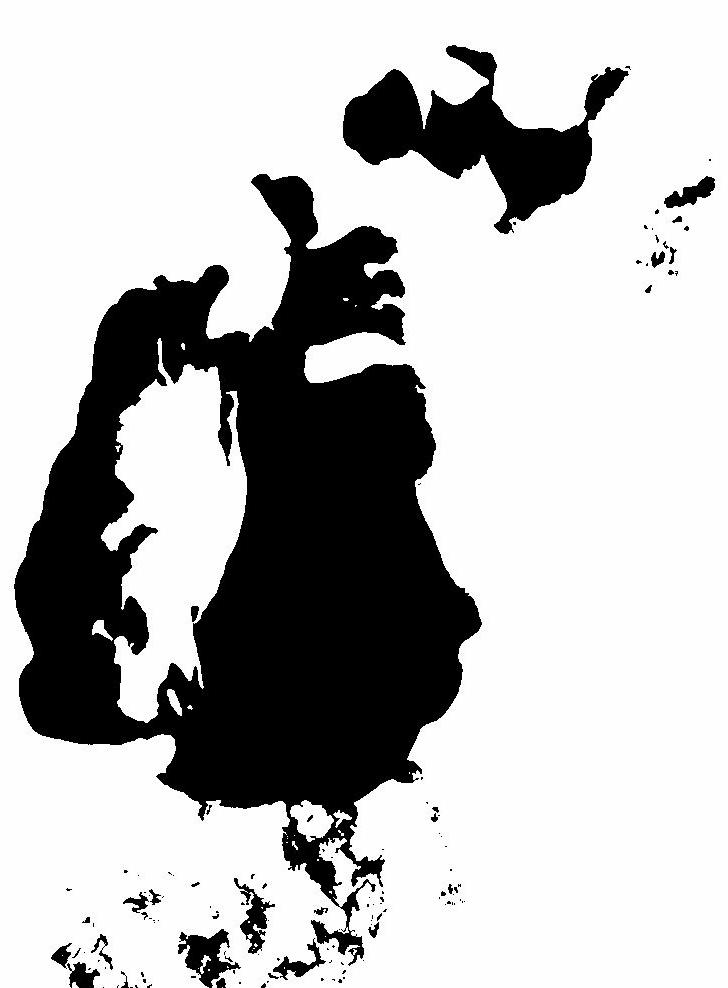
\includegraphics[width=\textwidth]{../img/1998w.jpg}
         \caption{}
         \label{fig:}
     \end{subfigure}
     \begin{subfigure}[b]{0.19\textwidth}
         \centering
         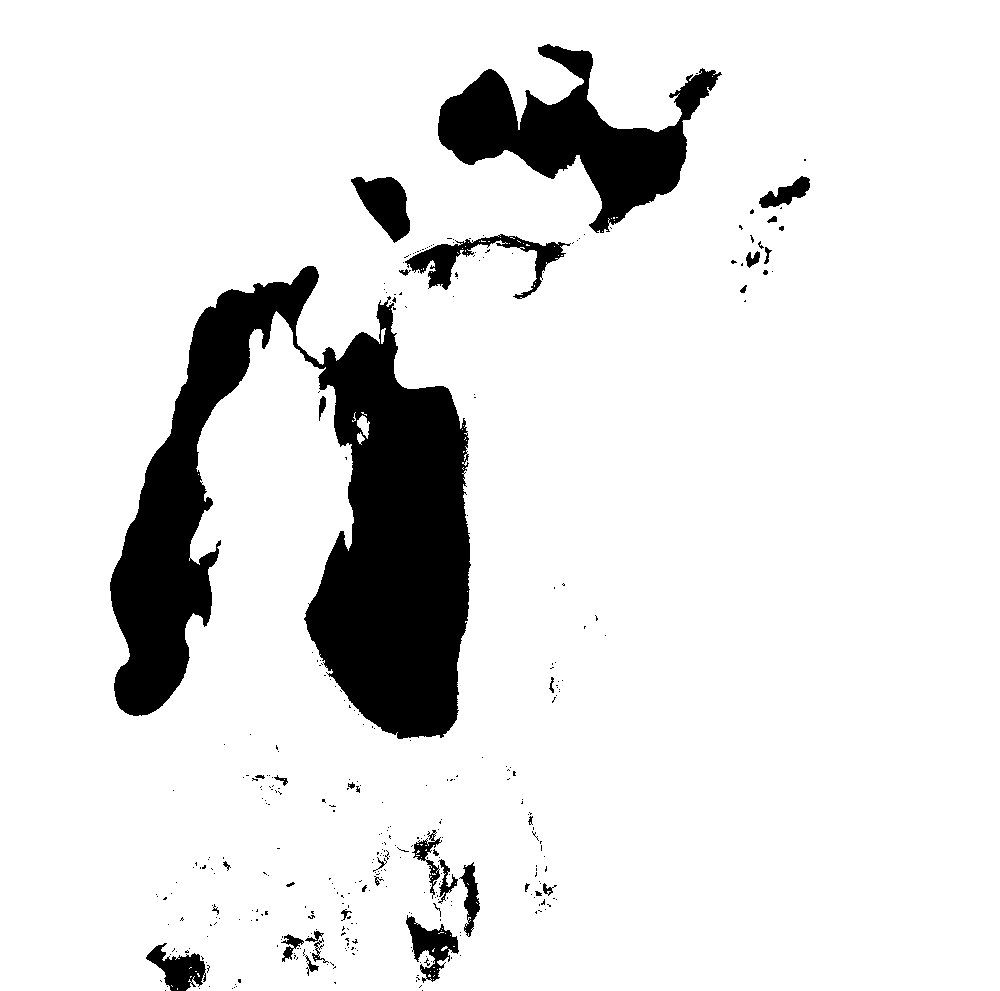
\includegraphics[width=\textwidth]{../img/2006w.jpg}
         \caption{}
         \label{fig:}
     \end{subfigure}
     \begin{subfigure}[b]{0.19\textwidth}
         \centering
         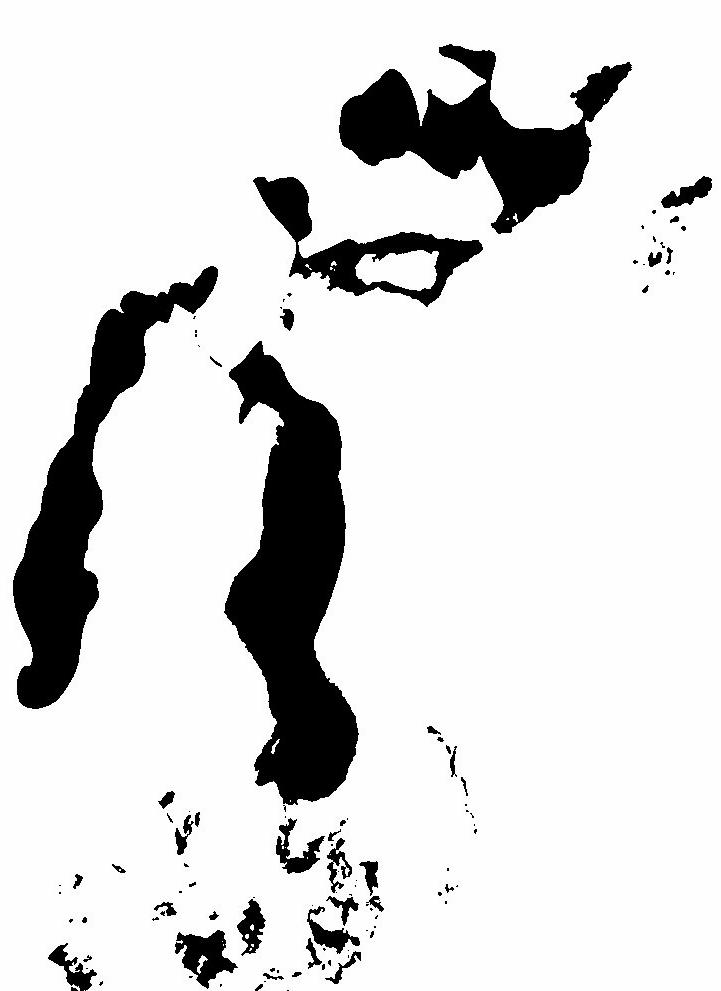
\includegraphics[width=\textwidth]{../img/2010w.jpg}
         \caption{}
         \label{fig:}
     \end{subfigure}
     \begin{subfigure}[b]{0.19\textwidth}
         \centering
         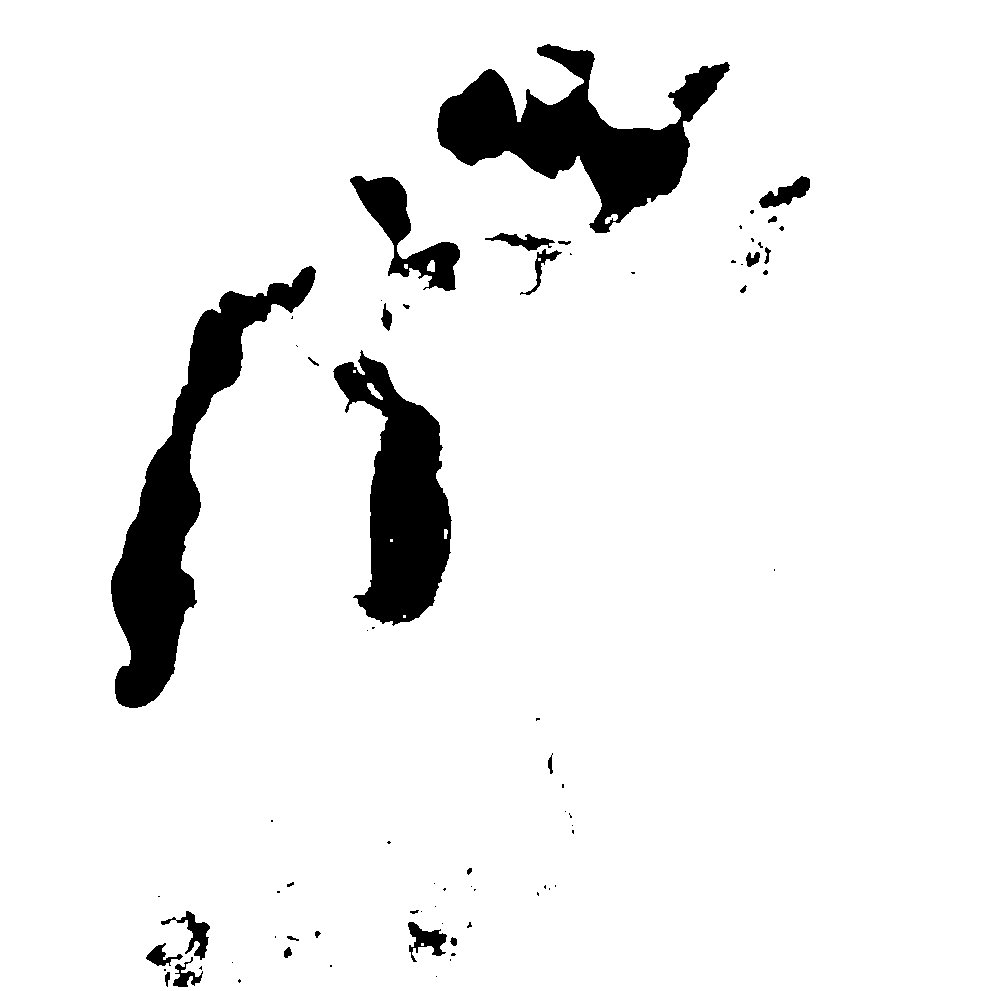
\includegraphics[width=\textwidth]{../img/2013w.jpg}
         \caption{}
         \label{fig:}
     \end{subfigure}
     \begin{subfigure}[b]{0.19\textwidth}
         \centering
         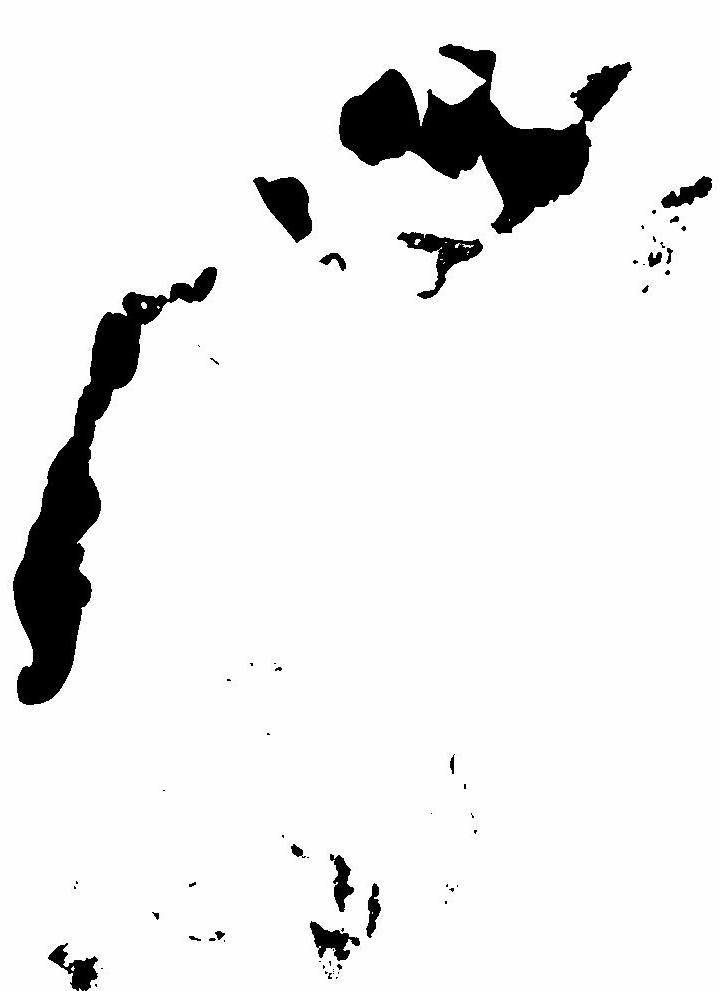
\includegraphics[width=\textwidth]{../img/2014w.jpg}
         \caption{}
         \label{fig:three sin x}
     \end{subfigure}
     \begin{subfigure}[b]{0.19\textwidth}
         \centering
         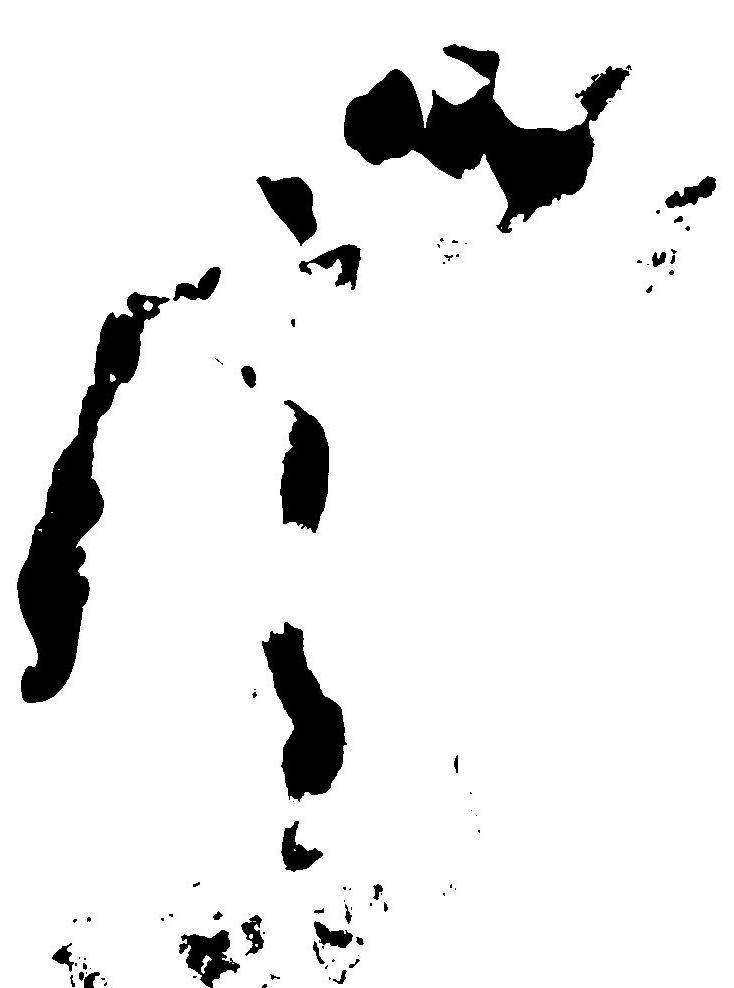
\includegraphics[width=\textwidth]{../img/2015w.jpg}
         \caption{}
         \label{fig:}
     \end{subfigure}
     \begin{subfigure}[b]{0.19\textwidth}
         \centering
         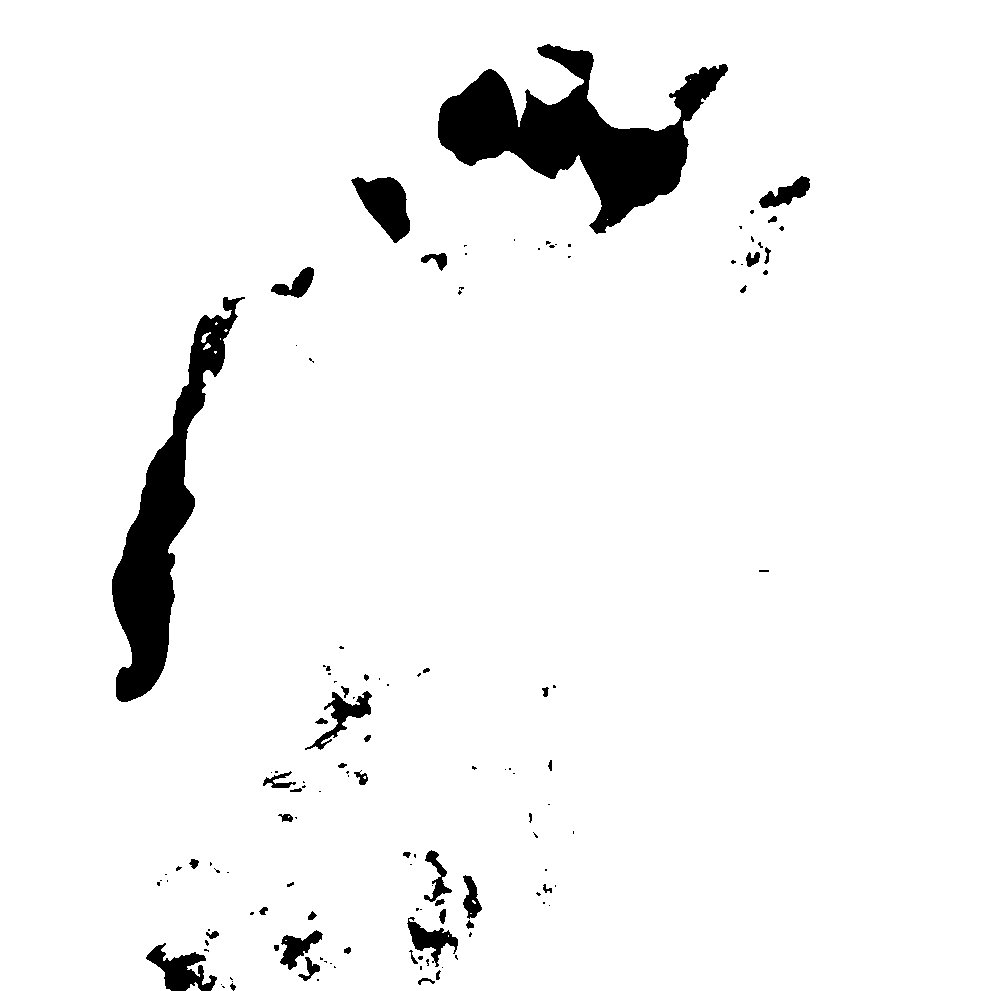
\includegraphics[width=\textwidth]{../img/2019w.jpg}
         \caption{}
         \label{fig:}
     \end{subfigure}
     \begin{subfigure}[b]{0.19\textwidth}
         \centering
         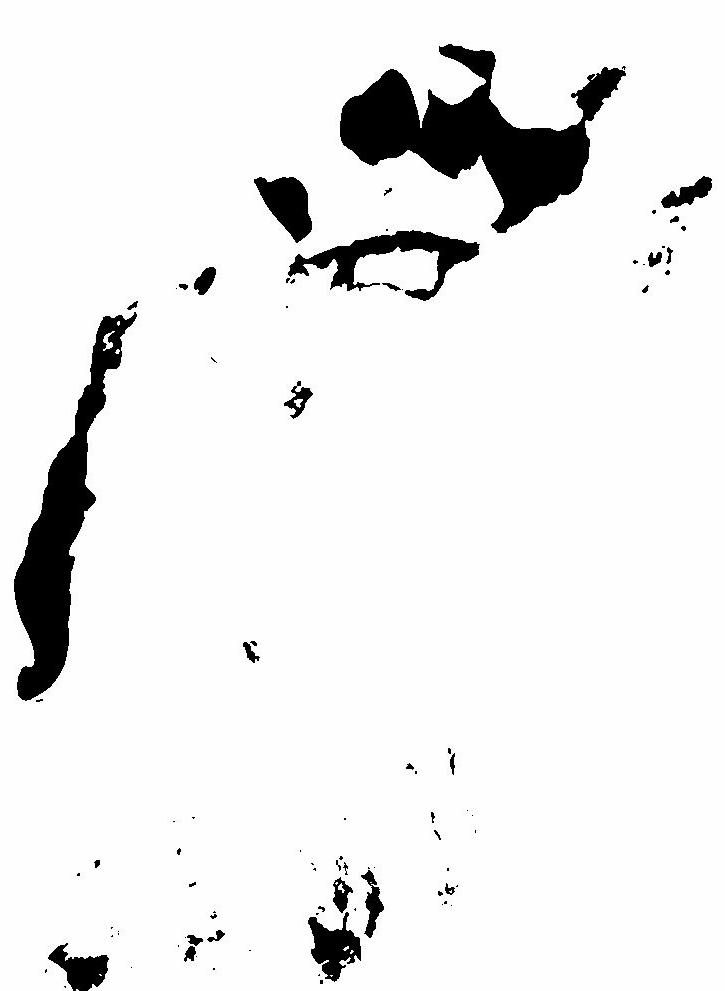
\includegraphics[width=\textwidth]{../img/2021w.jpg}
         \caption{}
         \label{fig:}
     \end{subfigure}
\end{figure}

\printbibliography

\end{document}
